\documentclass[10pt,aspectratio=169]{beamer}

% =============================================================
%  Presentación técnica del pipeline RAG
%  Proyecto: Tourism-Reports-LLM (Pueblos Mágicos)
% =============================================================

\usetheme{metropolis}
\usepackage[utf8]{inputenc}
\usepackage[spanish,es-tabla]{babel}
\usepackage{amsmath,amssymb,amsthm,bm}
\usepackage{mathtools}
\usepackage{bbm}
\usepackage{booktabs}
\usepackage{tikz}
\usepackage[table]{xcolor}
\usepackage{listings}
\usepackage{hyperref}
\usetikzlibrary{arrows.meta,positioning,shapes.geometric,fit,backgrounds,calc}

% --- Colores ---
\definecolor{cimatred}{HTML}{12393D}
\definecolor{primary}{HTML}{12393D}
\definecolor{accent}{HTML}{64293E}
\definecolor{soft}{HTML}{EAF1F8}
\definecolor{good}{HTML}{2E7D32}


% --- Listings (Python / JSON) ---
\lstdefinestyle{py}{
    basicstyle=\ttfamily\scriptsize,
    keywordstyle=\color{primary}\bfseries,
    commentstyle=\color{gray}\itshape,
    stringstyle=\color{accent},
    showstringspaces=false,
    breaklines=true,
    frame=single,
    rulecolor=\color{gray!40},
    language=Python,
}

% --- Macros matemáticos ---
\newcommand{\vq}{\mathbf{q}}
\newcommand{\vd}{\mathbf{d}}
\newcommand{\R}{\mathbb{R}}
\newcommand{\E}{\mathbb{E}}
\newcommand{\T}{^{\!\top}}
\DeclareMathOperator*{\argmax}{arg\,max}
\DeclareMathOperator*{\argmin}{arg\,min}
\DeclareMathOperator{\softmax}{softmax}
\DeclareMathOperator{\sgn}{sgn}

% --- TOC: secciones con círculo numerado ---
\setbeamertemplate{section in toc}{%
  \leavevmode%
  \tikz[baseline=-0.65ex]
    \node[circle, fill=accent, text=white,
          inner sep=2pt, font=\bfseries\scriptsize]
      {\inserttocsectionnumber};%
  \hspace{6pt}\inserttocsection\par%
}

% --- Metadatos ---
\title{Generación de Reportes Sintéticos sobre Pueblos Mágicos usando RAG}
\subtitle{Laboratorio ATLAS \\ Contacto: Dr. Miguel Ángel Álvarez Carmona}
\author{Gustavo Hernández Angeles}
\date{12 de mayo de 2026}

\begin{document}

% =============================================================
\maketitle
% =============================================================

\begin{frame}{Agenda}
	\begin{columns}[t]
		\column{0.48\textwidth}
		\tableofcontents[sections={1-5},hideallsubsections]
		\column{0.48\textwidth}
		\tableofcontents[sections={6-10},hideallsubsections]
	\end{columns}
\end{frame}

% =============================================================
\section{Introducción}
% =============================================================

\begin{frame}{Pueblos Mágicos}
	El programa \textbf{Pueblos Mágicos} (SECTUR, 2001) reconoce hoy a más de 170
	localidades mexicanas con valor simbólico, histórico o natural. Su propósito es
	\emph{revalorizar el patrimonio} y consolidar al turismo como motor de
	desarrollo económico regional.

	\medskip
	\begin{columns}[T,onlytextwidth]
		\column{0.52\textwidth}
		Una parte sustancial de la experiencia turística se documenta en línea:
		reseñas en \textbf{TripAdvisor, Google Maps o Booking}.
		Es retroalimentación nativa del visitante, pero su escala
		hace inviable el análisis manual sistemático.

		\column{0.46\textwidth}
		\centering
		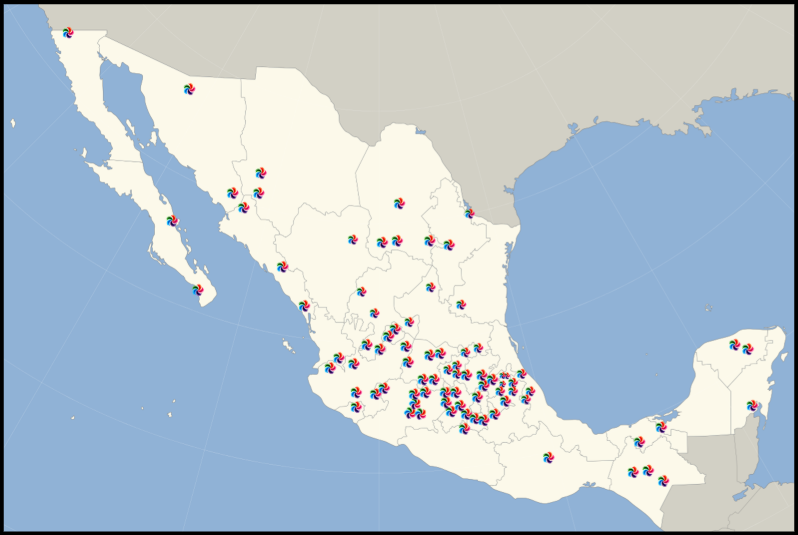
\includegraphics[width=\textwidth]{figures/mexico.png}
	\end{columns}
\end{frame}

\begin{frame}{Antecedentes \(\cdot\) Estado del arte}
	\textbf{Análisis automatizado de reseñas turísticas}
	\begin{itemize}\setlength\itemsep{2pt}
		\item Análisis de sentimiento y clasificación de polaridad sobre reseñas
		      con modelos tipo BERT/RoBERTa.
		\item \emph{Modelado de Tópicos} (LDA, BERTopic) y análisis basado en aspectos
		      para identificar atributos recurrentes de la experiencia:
		      limpieza, precio, atención, seguridad.
	\end{itemize}

	\medskip
	\textbf{Generación Aumentada por Recuperación (RAG)}
	\begin{itemize}\setlength\itemsep{2pt}
		\item Lewis \emph{et al.} (2020) introducen RAG: un LLM generador anclado
		      a evidencia externa mediante recuperación densa.
		\item Avances posteriores: \emph{reranking} con cross-encoders,
		      decodificación restringida y bucles de auto-corrección
		      (\emph{self-RAG}) que reducen alucinaciones.
		\item Salidas \textbf{estructuradas} (JSON-schema, Pydantic) permiten
		      integrar al LLM en flujos analíticos auditables y reproducibles.
	\end{itemize}
\end{frame}

\begin{frame}{Planteamiento del Problema}
	\textbf{Problema.}
	Cada Pueblo Mágico genera miles de reseñas anuales, dispersas en
	múltiples polaridades y categorías de negocio. Las autoridades
	turísticas requieren convertir ese \emph{big data} textual en reportes estratégicos accionables, pero hoy el proceso es
	manual, lento y difícil de escalar a más de 170 destinos.

	\medskip
	\begin{itemize}\setlength\itemsep{3pt}
		\item ¿Cómo \textbf{sintetizar} cientos de miles de opiniones sin perder
		      evidencia ni introducir alucinaciones del LLM?
		\item ¿Cómo separar la \textbf{atribución pública} (infraestructura,
		      señalización, servicios básicos, seguridad) de la
		      \textbf{atribución privada} (gestión y calidad del servicio)?
		\item ¿Cómo entregar un diagnóstico
		      \textbf{auditable, reproducible y trazable} a la reseña fuente?
	\end{itemize}
\end{frame}

\begin{frame}{Planteamiento del Problema \(\cdot\) Relevancia}
	\begin{columns}[T,onlytextwidth]
		\column{0.55\textwidth}
		\textbf{¿Por qué importa?}
		\begin{itemize}\setlength\itemsep{3pt}
			\item El turismo representa cerca del \textbf{8.5\,\% del PIB
				      mexicano}; los Pueblos Mágicos concentran un flujo
			      creciente de visitantes nacionales e internacionales.
			\item Las decisiones de \textbf{inversión pública} (accesos,
			      señalética, seguridad) compiten con la mejora de la
			      \textbf{oferta privada} (capacitación, hotelería,
			      gastronomía); priorizar mal es costoso.
			\item La opinión de los turistas ya contiene una señal para priorizar;
			      el cuello de botella es el costo de análisis.
		\end{itemize}

		\column{0.42\textwidth}
		\centering
		\begin{tikzpicture}[font=\footnotesize, node distance=14mm]
			\node[draw=gray!50, fill=gray!10, rounded corners=4pt,
				minimum width=30mm, minimum height=16mm, align=center] (docs)
			{Reseñas\\masivas};
			\node[draw=accent, fill=accent!12, rounded corners=4pt,
				minimum width=30mm, minimum height=16mm, align=center,
				below=18mm of docs] (report)
			{Reporte\\accionable};
			\draw[-{Stealth[length=4mm]}, very thick, accent, line width=3pt]
			(docs) -- (report);
		\end{tikzpicture}
	\end{columns}
\end{frame}

% =============================================================
\section{Conjunto de Datos}
% =============================================================

\begin{frame}{Conjunto de Datos}
	\textbf{Descripción.} El conjunto de datos consta de \textbf{+300\,000} reseñas de turistas
	sobre negocios / atracciones ubicados en los Pueblos Mágicos de México.
	Cada registro cuenta con:

	\begin{itemize}
		\item Título y cuerpo de la reseña.
		\item Nombre del negocio.
		\item Tipo de Negocio (Hotel, Restaurante, Atracción).
		\item Pueblo Mágico.
		\item Calificación.
	\end{itemize}

	\medskip
	\begin{table}[h]
		\centering
		\scriptsize
		\setlength{\tabcolsep}{5pt}
		\renewcommand{\arraystretch}{1.3}
		\begin{tabular}{|p{0.36\textwidth}|p{0.17\textwidth}|p{0.17\textwidth}|p{0.12\textwidth}|}
			\hline
			\rowcolor{accent!80}
			\color{white}\textbf{Titulo y Reseña}         &
			\color{white}\textbf{Tipo de Negocio}         &
			\color{white}\textbf{Pueblo Mágico}           &
			\color{white}\textbf{Calificación}                                             \\
			\hline
			Relax \%100: Playa limpia buenos servicios\ldots\ nos deja mal sabor de boca
			fue el hotel por su falta de compromiso\ldots & Atracción & Isla Mujeres & 5/5 \\
			\hline
		\end{tabular}
	\end{table}
\end{frame}

% =============================================================
\section{Objetivos y Solución Propuesta}
% =============================================================

\begin{frame}{Objetivos}
	\textbf{Objetivo General}\\[4pt]
	Desarrollar un sistema basado en modelos grandes de lenguaje (LLM) para generar
	automáticamente reportes sintéticos de alta calidad sobre la percepción y la experiencia
	del turista en Pueblos Mágicos de México, a partir de colecciones masivas de reseñas.

	\bigskip
	\textbf{Objetivos Específicos}
	\begin{itemize}
		\item Diseñar y construir una base de conocimiento para el LLM a partir del conjunto
		      de datos.
		\item Implementar un flujo de trabajo para la generación de reportes que utilice la
		      base de conocimiento, además de guiar al LLM en la estructuración y síntesis
		      del contenido.
		\item Evaluar la calidad, coherencia y factualidad de los reportes sintéticos generados.
	\end{itemize}
\end{frame}

\begin{frame}{Alcance del proyecto}
	\textbf{Lo que se entrega.} Un prototipo funcional a nivel de
	flujo de trabajo, el cual es ejecutable desde la línea de comandos.

	\medskip
	\textbf{Lo que queda fuera del alcance.}
	\begin{itemize}\setlength\itemsep{3pt}
		\item No contempla el \textbf{despliegue en producción} ni el
		      desarrollo de una \textbf{interfaz de usuario} (web, móvil o
		      escritorio) para consumo por usuarios finales.
		\item No incluye esfuerzos de ingeniería de software orientados a
		      \textbf{escalabilidad, monitoreo, autenticación} u otras
		      consideraciones propias de un producto listo para uso final.
		\item El resultado es un \textbf{prototipo a nivel de flujo de trabajo},
		      no una aplicación desplegada.
	\end{itemize}
\end{frame}

\begin{frame}{Solución Propuesta}
	\centering
	\begin{tikzpicture}[
		font=\scriptsize,
		node distance=4mm and 6mm,
		every node/.style={align=center},
		phase/.style={rectangle, rounded corners=3pt, draw=primary, thick,
				fill=white, minimum width=26mm, minimum height=12mm,
				inner sep=2pt, font=\scriptsize\bfseries},
		arr/.style={-{Stealth[length=2mm]}, thick, primary},
		stagebox/.style={rectangle, rounded corners=5pt, very thick,
				inner sep=5pt},
		]

		% Etapa 1 — RAG: construcción vectorial
		\node[phase] (chunk)  {Fragmentación de \\ Textos};
		\node[phase, right=of chunk] (emb)    {Embedding \\ \scriptsize SBERT-es};
		\node[phase, right=of emb]   (hnsw)   {Indexado HNSW};

		% Etapa 1 — RAG: retrieval + reranking
		\node[phase, below=10mm of chunk] (filt)  {Filtros\\meta\,$\mathcal{F}$};
		\node[phase, right=of filt]       (ann)   {Approximate Nearest \\Neighbors};
		\node[phase, right=of ann]        (ce)    {Reranking \\ Cross-encoder};

		% Etapa 2 — Generación
		\node[phase, below=10mm of filt]  (gen)   {Elección de LLM};
		\node[phase, right=of gen]        (cd)    {Constrained \\ decoding};
		\node[phase, right=of cd]         (out)   {Salida\\Pydantic};

		% Etapa 3 — Evaluación
		\node[phase, right=20mm of out]   (audit) {Auditoría};

		% Cajas de etapa (fondo)
		\begin{scope}[on background layer]
			\node[stagebox, draw=primary, fill=primary!8,
				fit=(chunk)(emb)(hnsw)(filt)(ann)(ce)] (rag_box) {};
			\node[stagebox, draw=accent, fill=accent!8,
				fit=(gen)(cd)(out)] (gen_box) {};
			\node[stagebox, draw=good, fill=good!8,
				fit=(audit)] (eval_box) {};
		\end{scope}

		% Etiquetas de etapa
		\node[right=4pt of rag_box, font=\scriptsize\bfseries, primary]
		{Etapa 1: RAG};
		\node[above=2pt of gen_box,  font=\scriptsize\bfseries, accent]
		{Etapa 2: Generación};
		\node[above=2pt of eval_box, font=\scriptsize\bfseries, good]
		{Etapa 3: Evaluación};

		% Conexiones horizontales
		\draw[arr] (chunk) -- (emb);
		\draw[arr] (emb)   -- (hnsw);
		\draw[arr] (filt)  -- (ann);
		\draw[arr] (ann)   -- (ce);
		\draw[arr] (gen)   -- (cd);
		\draw[arr] (cd)    -- (out);

		% Conexiones inter-etapa
		\draw[arr] (hnsw.south) -- ++(0,-2mm) -| (filt.north);
		\draw[arr] (ce.south)   -- ++(0,-2mm) -| (gen.north);
		\draw[arr] (out)        -- (audit);
		\draw[arr, dashed, good]
		(audit.south) -- ++(0,-4mm) -|
		node[pos=0.25, below, font=\scriptsize\itshape]{Re-intento $\le 3$}
		(gen.south);

	\end{tikzpicture}

	\footnotesize
	\textbf{1.~RAG:} Construcción vectorial \textbullet\ Recuperación
	\textbf{2.~Generación Estructurada} LLM + Estructura de salida
	\textbf{3.~Evaluación:} Auditoría con auto-corrección
\end{frame}

% =============================================================
\section{Marco Teórico y Metodología}
% =============================================================

\begin{frame}[fragile]{Notación y datos del corpus}
	\begin{columns}[T,onlytextwidth]
		\column{0.55\textwidth}
		\textbf{Corpus.} Reseñas TripAdvisor (RESTMEX) clasificadas por
		tipo $\in\{\text{Hotel, Restaurant, Attractive}\}$.

		\medskip
		\textbf{Volumen indexado.}
		\begin{itemize}
			\item $N = 1{,}067{,}981$ fragmentos de texto
			\item $\sim 5.1$ GB en disco (ChromaDB persistente)
			\item Dim. del embedding $d = 768$
		\end{itemize}

		\medskip
		\textbf{Notación.}
		\begin{itemize}
			\item $\vq \in \R^d$: embedding de la consulta
			\item $\vd_i \in \R^d$: embedding del chunk $i$
			\item $\mathcal{F}$: filtro sobre metadatos
			      (\texttt{town, type, polarity, year, $\dots$})
			\item $\mathcal{D}_\mathcal{F} = \{\vd_i : m_i \models \mathcal{F}\}$
		\end{itemize}

		\column{0.45\textwidth}
		\textbf{Metadatos por chunk}
		\scriptsize
		\begin{lstlisting}[style=py,language=Python]
{
  "town":     "Isla_Mujeres",
  "type":     "Restaurant",
  "polarity": 4,
  "place":    "...",
  "month":    7,
  "year":     2023,
  "source_id":  "...",
  "chunk_index": 2,
}
\end{lstlisting}
	\end{columns}
\end{frame}

\begin{frame}{RAG: Generación aumentada por recuperación}
	\textbf{Conocimiento limitado de los LLMs.}
	\begin{itemize}
		\item Un LLM aprende de un corpus general; su \textbf{memoria paramétrica}
		      cubre mal dominios especializados y hechos locales.
		\item Ante vacíos de información, tiende a \textbf{alucinar}: produce
		      texto plausible pero falso, sin marcar la incertidumbre.
		\item \emph{Ejemplo.} Preguntar ``¿qué problemas reportan los turistas
		      en Santiago, N.L.?'' El modelo no vio reseñas turísticas de
		      ese Pueblo Mágico durante el entrenamiento, así que es muy
		      probable que \textbf{invente} quejas y atribuciones.
	\end{itemize}

	\medskip
	\textbf{Idea principal.} En lugar de confiar en lo que el modelo
	``recuerda'', \textbf{recuperamos} evidencia relevante (reseñas reales,
	filtradas por pueblo y tipo de negocio) y se la entregamos como
	contexto. La generación queda \textbf{anclada a documentos verificables}
	en vez de a memoria difusa.
\end{frame}

% =============================================================
% CONSTRUCCION DE LA BASE VECTORIAL
%
\section*{1. Construcción de la base vectorial}
% =============================================================

\subsection{1. Construcción de la base vectorial}

\begin{frame}{1.1 Fragmentación: intuición}
	\textbf{¿Por qué fragmentar?}
	\begin{itemize}
		\item Los \emph{transformers} de embedding tienen ventana finita
		      (típicamente $\le 512$ tokens). Documentos largos se
		      \emph{truncarían}.
		\item Un embedding por documento entero \textbf{promedia señales} de
		      múltiples tópicos; el coseno entre $\vq$ y un vector que mezcla
		      ``servicio + ubicación + ruido'' se diluye.
		\item Granularidad más fina $\Rightarrow$ mejor \textbf{recall}
		      semántico (cada queja, cada elogio, vive en un chunk propio).
	\end{itemize}

	\medskip
	\textbf{Trade-off.} Chunks demasiado cortos pierden contexto
	sintáctico; demasiado largos diluyen relevancia. Para reseñas (texto
	corto y tópico-denso) se elige una ventana pequeña.
\end{frame}

% \begin{frame}[fragile]{1.1 Fragmentación: formulación y configuración}
% 	% \textbf{Splitter recursivo.} Sea $T$ el texto y
% 	% $S = (s_1, s_2, \dots, s_m)$ una jerarquía de separadores. El algoritmo
% 	% recursivo es:
% 	% \[
% 	% 	\mathrm{split}(T, S) =
% 	% 	\begin{cases}
% 	% 		\{T\}                                  & \text{si } |T| \le L \\[2pt]
% 	% 		\bigcup_j \mathrm{split}(T_j, S_{2:m}) & \text{si } |T| > L,\
% 	% 		T = T_1 \oplus s_1 \oplus T_2 \oplus \cdots
% 	% 	\end{cases}
% 	% \]
% 	% con \emph{merge} posterior que respeta longitud máxima $L$ y
% 	% solapamiento $o$.

% 	\medskip
% 	\textbf{Configuración del proyecto:}
% 	\begin{itemize}
% 		\item $L = 200$ caracteres, $o = 50$ (ratio $25\%$)
% 		\item $S = (\texttt{"\textbackslash n\textbackslash n", "\textbackslash n", ". ", " ", ""})$
% 		\item Implementación: \texttt{RecursiveCharacterTextSplitter}
% 		      (LangChain)
% 	\end{itemize}

% 	\medskip
% 	\textbf{Justificación.} Las reseñas RESTMEX rara vez superan 1–2
% 	párrafos; $L=200$ atomiza al nivel de \emph{frase larga / micro-aspecto},
% 	y el solape $o=50$ evita cortar entidades en frontera.

% \end{frame}

% --- Ejemplo de fragmentación ---
\begin{frame}{1.1 Fragmentación: ejemplo real}
	\vspace{\fill}
	\begin{columns}[c]
		\column{0.50\textwidth}
		\begin{tikzpicture}[font=\tiny, >=Stealth]
			% --- Barra: texto original ---
			\node[font=\scriptsize\bfseries] at (4.0, 5.15) {Reseña original};
			\fill[gray!20]    (0.0, 4.65) rectangle (8.0, 5.00);
			\draw[gray!60]    (0.0, 4.65) rectangle (8.0, 5.00);
			\node[font=\tiny, text=black!80] at (4.0, 4.825)
			{\textit{``Pasamos una semana aquí\ldots La playa es bonita\ldots El servicio es amable\ldots''}};

			% --- Fragmento 1 ---
			\fill[primary!25] (0.0, 3.30) rectangle (4.8, 3.75);
			\draw[primary!70, thick] (0.0, 3.30) rectangle (4.8, 3.75);
			\node[font=\tiny\bfseries] at (2.4, 3.525) {Fragmento 1};

			% --- Fragmento 2 ---
			\fill[accent!20]  (1.6, 2.20) rectangle (6.4, 2.65);
			\draw[accent!70,  thick] (1.6, 2.20) rectangle (6.4, 2.65);
			\node[font=\tiny\bfseries] at (4.0, 2.425) {Fragmento 2};

			% --- Fragmento 3 ---
			\fill[blue!15]    (3.2, 1.10) rectangle (8.0, 1.55);
			\draw[blue!50,    thick] (3.2, 1.10) rectangle (8.0, 1.55);
			\node[font=\tiny\bfseries] at (5.6, 1.325) {Fragmento 3};

			% Líneas de guía verticales
			\foreach \x/\bot in {0.0/3.30, 4.8/3.30, 1.6/2.20, 6.4/2.20, 3.2/1.10, 8.0/1.10}{
					\draw[dashed, gray!45, thin] (\x, 4.65) -- (\x, \bot);
				}
		\end{tikzpicture}

		\column{0.50\textwidth}
		\centering
		{\tiny\setlength{\fboxsep}{3pt}%
			\colorbox{primary!25}{\parbox{4.8cm}{%
					\textbf{Fragmento 1}\\[1pt]
					\textit{``Pasamos una semana aquí, recientemente,
						y nos gustó mucho el lugar. Puedo ver
						por qué se llama el mejor hotel de la isla\ldots''}
				}}

			\vspace{4pt}
			\colorbox{accent!20}{\parbox{4.8cm}{%
					\textbf{Fragmento 2}\\[1pt]
					\textit{``\ldots\ Realmente la única pega es la
						ubicación, lo que puede ser una ventaja
						si no quieres estar alrededor de los
						centros de la isla\ldots''}
				}}

			\vspace{4pt}
			\colorbox{blue!15}{\parbox{4.8cm}{%
					\textbf{Fragmento 3}\\[1pt]
					\textit{``\ldots\ La playa es bonita, exclusiva
						para el hotel, y las piscinas son de calidad.
						El servicio es amable y satisfactorio\ldots''}
				}}
		}
	\end{columns}
\end{frame}

\subsection{1.2 Embeddings: SBERT en español}

\begin{frame}{1.2 Embeddings de texto para similaridad}
	\textbf{Modelo Bi-Encoder:} \texttt{hiiamsid/sentence\_similarity\_spanish\_es}.
	Fine-tuning de \textbf{BETO} (BERT entrenado sobre corpus en español) para similaridad de textos.

	\medskip
	\textbf{Función de embedding.}
	Dado un texto $x$ con tokens $(t_1,\dots,t_n)$ y representaciones por
	capa $\mathbf{H} \in \R^{n \times d}$ (con $d=768$), se aplica
	\emph{mean pooling} con máscara de atención $\mathbf{a}\in\{0,1\}^n$:
	\[
		f(x) \;=\; \frac{\sum_{i=1}^{n} a_i\, \mathbf{H}_i}{\sum_{i=1}^{n} a_i}
		\;\in\; \R^{768}.
	\]

	Además, se aplica una normalización L2 a los embeddings para que la distancia coseno sea solo un producto punto.

	\textbf{Objetivo de entrenamiento.}
	Para pares $(a,b)$ con etiqueta $s$ (similitud), se minimiza un
	\emph{cosine MSE}:
	\[
		\mathcal{L}(a,b,s) \;=\; \bigl(\,\cos(f(a), f(b)) - s\,\bigr)^2,
	\]
\end{frame}

\begin{frame}{Ejemplo de recuperación}
	\textbf{Consulta:} ``Problemas con acceso infraestructura, señalización, guía o seguridad.'' \\ \vspace{0.1cm}
	\textbf{Fragmentos relevantes:}
	\begin{itemize}
		\item ``manejan y no respetan al peatón y/o el orden de la circulación''
		\item ``Algunos sitios son algo peligrosos. Ten cuidado''
		\item ``y puesto que las aceras son demasiado estrechas o obstruida, es una danza hostil''
		\item ...
	\end{itemize}
\end{frame}

\subsection{1.3 Indexado HNSW}

\begin{frame}{1.3 El problema: k-NN exacto es prohibitivo}
	\textbf{k-NN exacto} para una consulta $\vq$:
	\[
		\mathcal{C}_K^{*} \;=\;
		\argmax_{\substack{S \subseteq \mathcal{D} \\ |S|=K}}
		\sum_{\vd \in S} \cos(\vq,\vd),
		\qquad
		\text{costo: } \mathcal{O}(N\cdot d).
	\]

	\textbf{Magnitud.} Con $N=1{,}067{,}981$ y $d=768$:
	\[
		N \cdot d \;\approx\; 8.2 \times 10^{8}\ \text{flops por consulta},
	\]
	incompatible con latencia interactiva en CPU/GPU comerciales.

	\medskip
	\textbf{Solución: ANN (Approximate Nearest Neighbors).}\\
	Aceptamos un recall ligeramente $<1$ a cambio de complejidad esperada
	sub-lineal. El algoritmo \textit{Mundo Pequeño Nevagable Jerárquico} (HNSW) (Malkov \& Yashunin, 2018) es el
	estado del arte para similaridad coseno/euclidiana en dimensiones moderadas.
\end{frame}

\begin{frame}{1.3 HNSW: Construcción de la base de conocimiento}
	\textbf{Idea.} Combinar dos estructuras:
	\begin{itemize}
		\item \textbf{Skip-lists} $\to$ jerarquía probabilística de capas
		      con distintas densidades.
		\item \textbf{Small-world graphs} (Kleinberg) $\to$ enlaces cortos
		      (vecinos cercanos) + enlaces largos (saltos).
	\end{itemize}

	\medskip
	\textbf{Asignación de capas.} Cada nodo representa un fragmento de texto. A cada nodo $v$ se le asigna un nivel
	máximo $\ell(v)$ con distribución geométrica truncada
	\[
		P(\ell = k) \;=\; (1-p)\,p^{k},
		\qquad p = \frac{1}{\ln M},
	\]
	donde $M$ es el número objetivo de vecinos por nodo y por capa.
	La esperanza es $\E[\ell] = p/(1-p) = 1/(\ln M - 1)$, produciendo
	una pirámide con muy pocos nodos en capas altas.

	\medskip
	\textbf{Garantía estructural.} El grafo de la capa 0 contiene a
	\emph{todos} los nodos; las capas superiores actúan como
	\emph{índices gruesos}.
\end{frame}

\begin{frame}{1.3 HNSW: Construcción}
	\begin{figure}
		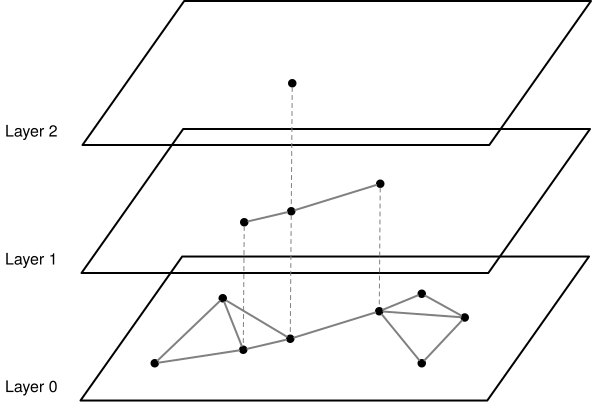
\includegraphics[width=0.6\textwidth]{figures/06-hnsw-architecture.pdf}
	\end{figure}
\end{frame}

\begin{frame}{1.3 HNSW: algoritmo de búsqueda}
	\textbf{Greedy descent multi-capa.} Sea $L_{\max}$ la capa más alta y
	$\vq$ la consulta:
	\begin{enumerate}
		\item Iniciar en el punto de entrada $e \in V_{L_{\max}}$.
		\item Para $\ell = L_{\max}, L_{\max}-1, \dots, 1$:
		      avanzar greedy a
		      \[
			      e \leftarrow \argmin_{u \in \mathcal{N}_\ell(e)\cup\{e\}}
			      \|\vq - \mathbf{u}\|,
		      \]
		      hasta convergencia local en la capa.
		\item En la capa 0, ejecutar búsqueda con \emph{cola de prioridad de
			      tamaño} \texttt{ef\_search}: mantener un conjunto candidato
		      $\mathcal{C}$ y un conjunto resultado $\mathcal{W}$;
		      expandir hasta que ningún candidato mejore al peor de
		      $\mathcal{W}$.
		\item Devolver los $K$ más cercanos en $\mathcal{W}$.
	\end{enumerate}

	\medskip
	\textbf{Complejidad esperada.}
	\[
		\mathcal{O}\bigl(\log N\bigr)\ \text{pasos por consulta},
	\]
	con constante dominada por $M \cdot \texttt{ef\_search}$.
\end{frame}

\begin{frame}{1.3 HNSW: Consulta}
	\begin{figure}
		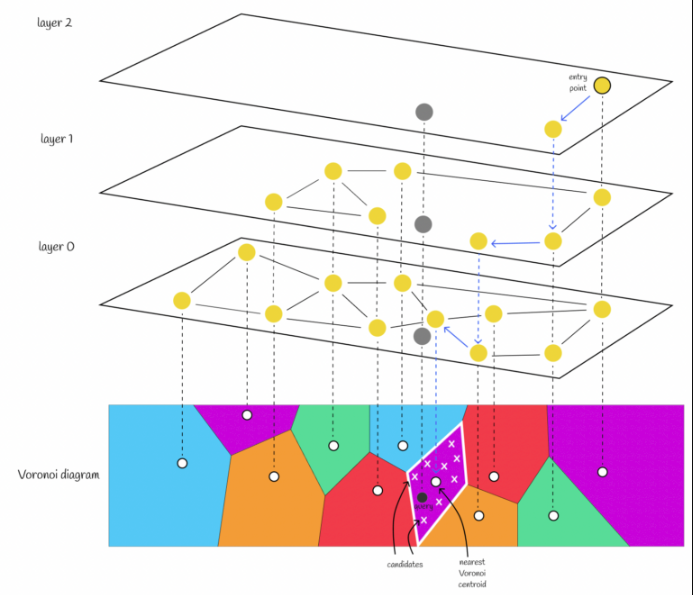
\includegraphics[height=0.8\textheight]{figures/hnsw_consulta.png}
	\end{figure}
\end{frame}

% =============================================================
\section*{2. Recuperación}
% =============================================================

\begin{frame}{2. Recuperación: filtrado de datos}
	\textbf{Problema.} Dada una consulta $\vq$ y un filtrado de metadatos
	$\mathcal{F}$, recuperar
	\[
		\mathcal{C}_K \;=\;
		\argmax_{\substack{S \subseteq \mathcal{D}_{\mathcal{F}} \\ |S|=K}}
		\sum_{\vd \in S} \cos(\vq,\vd),
		\qquad
		\mathcal{D}_{\mathcal{F}} \subseteq \mathcal{D}.
	\]

	\textbf{Pre-filtrado por metadatos.} ChromaDB compone una cláusula
	\texttt{where} estructurada:
	\begin{align*}
		\mathcal{F} \;=\;\  & \bigl\{ \texttt{town} = \text{``Isla\_Mujeres''} \bigr\}\
		\land                                                                                \\
		                    & \bigl\{ \texttt{type} \in \{\text{Hotel, Restaurant}\}\bigr\}\
		\land\ \cdots
	\end{align*}
	La estrategia de pre-filtrado restringe el subgrafo HNSW
	a $\mathcal{D}_{\mathcal{F}}$ \emph{antes} de la expansión greedy.
	% , en
	% contraste con \emph{post-filtering} (que descarta tras buscar y
	% sufre baja densidad efectiva si $\mathcal{F}$ es restrictivo).

	\medskip
	\textbf{Razón.} Las consultas siempre se anclan a un Pueblo Mágico
	y un tipo de negocio; sin pre-filtrado, el ANN devolvería resultados
	fuera de dominio.
\end{frame}

\begin{frame}{2. Recuperación en dos pasos: recuperación y re-ranking}
	\textbf{Estrategia.} En lugar de pedir al bi-encoder los $K$ finales,
	se sobre-recupera un factor $\alpha = 3$:
	\[
		\mathcal{C}^{(1)} \;=\;
		\text{top-}(\alpha K)_{\vd \in \mathcal{D}_{\mathcal{F}}}
		\cos(\vq,\vd)
		\quad\text{(bi-encoder, HNSW)}.
	\]
	Después, el cross-encoder $g$ reordena $\mathcal{C}^{(1)}$ y
	\[
		\mathcal{C}_K \;=\;
		\text{top-}K_{\vd \in \mathcal{C}^{(1)}}
		g(\vq, \vd).
	\]

	\textbf{¿Por qué $\alpha=3$?} Compromiso entre:
	\begin{itemize}
		\item \textbf{Recall.} El bi-encoder es rápido pero
		      ruidoso. Con $\alpha=3$, la probabilidad de que los documentos relevantes estén
		      en $\mathcal{C}^{(1)}$ aumenta notoriamente.
		\item \textbf{Costo del reranker.} Cada par $(\vq,\vd)$ requiere un
		      forward pass completo del cross-encoder; $\alpha=3$ mantiene la
		      latencia del re-ranking acotada.
	\end{itemize}

	\medskip
	\textbf{Idea clave.} Bi-encoder filtra eficientemente,
	el cross-encoder discrimina con alta precisión sobre un conjunto pequeño.
\end{frame}

% -------------------------------------------------------------
\begin{frame}{2. Re-ranking — ejemplo con reseñas de hotel}
	\vspace{-0.15em}
	\begin{center}
		\small\textbf{Consulta:}\;
		\textit{``¿Cómo es el desayuno en los hoteles?''}
		\quad{\scriptsize ($\alpha=3,\;K=3$)}
	\end{center}
	\vspace{-0.45em}
	\centering
	\begin{tikzpicture}[
		box/.style={rectangle, rounded corners=2pt,
				minimum width=5.3cm, minimum height=0.56cm,
				text width=5.0cm, font=\tiny, align=left,
				inner sep=3pt},
		rel/.style={box, fill=good!12, draw=good!70},
		irr/.style={box, fill=gray!10, draw=gray!40},
		hdr/.style={font=\scriptsize\bfseries, align=center},
		arr/.style={-{Stealth[length=4pt]}, thick, good,
		shorten >=2pt, shorten <=2pt},
		]

		% ---- Columna izquierda: bi-encoder ----
		\node[hdr] at (2.9, 0.15) {Bi-encoder — 6 candidatos};

		\node[irr] (b1) at (2.9,-0.50)
		{\#1\;sim\,=\,0.82\enspace``La cocina disponible no tiene\ldots''};
		\node[rel] (b2) at (2.9,-1.10)
		{\#2\;sim\,=\,0.79\enspace``Desayuno buffet: fruta fresca y café de olla\ldots''};
		\node[irr] (b3) at (2.9,-1.70)
		{\#3\;sim\,=\,0.77\enspace``El atún estaba muy bueno\ldots''};
		\node[rel] (b4) at (2.9,-2.30)
		{\#4\;sim\,=\,0.75\enspace``Huevos rancheros del desayuno, lo mejor\ldots''};
		\node[irr] (b5) at (2.9,-2.90)
		{\#5\;sim\,=\,0.73\enspace``Un buen lugar para comer en la mañana\ldots''};
		\node[rel] (b6) at (2.9,-3.50)
		{\#6\;sim\,=\,0.71\enspace``Menú incluye opciones veganas en desayuno\ldots''};

		% ---- Columna derecha: cross-encoder ----
		\node[hdr] at (10.1, 0.15) {Cross-encoder — top-3 final};

		\node[rel] (c1) at (10.1,-0.50)
		{\#1\;rel\,=\,0.94\enspace``Desayuno buffet: fruta fresca y café de olla\ldots''};
		\node[rel] (c2) at (10.1,-1.10)
		{\#2\;rel\,=\,0.91\enspace``Huevos rancheros del desayuno, lo mejor\ldots''};
		\node[rel] (c3) at (10.1,-1.70)
		{\#3\;rel\,=\,0.88\enspace``Menú incluye opciones veganas en desayuno\ldots''};

		% ---- Flechas (los relevantes ascienden) ----
		\draw[arr] (b2.east) to[out=0, in=180] (c1.west);
		\draw[arr] (b4.east) to[out=0, in=180] (c2.west);
		\draw[arr] (b6.east) to[out=0, in=180] (c3.west);

		% ---- Leyenda ----
		\node[font=\tiny, text=gray!70, align=center] at (6.5,-4.2)
		{Verde: reseña relevante para la consulta.\quad
			Gris: reseña fuera de tema (eliminada).};

	\end{tikzpicture}
\end{frame}

% =============================================================
% =============================================================

% =============================================================
\section*{4. Generación de texto restringida}
% =============================================================

\begin{frame}{4. Generación: el problema de la salida estructurada}
	% \textbf{Modelo generador.}
	% \[
	% 	\texttt{meta-llama/Llama-3.1-8B-Instruct},\qquad
	% 	\tau = 0\ \text{(decodificación greedy)}.
	% \]
	% Eliminando varianza estocástica:
	% \[
	% 	y_t \;=\; \argmax_{v \in \mathcal{V}}\,
	% 	p_\theta\bigl(v \mid y_{<t}, \vq, \mathcal{C}_K\bigr).
	% \]

	\textbf{Reto.} Las fases posteriores del flujo de trabajo consumen
	\emph{objetos tipados} (Formato de salida JSON). Un parser que
	``espera JSON'' falla con cualquier desviación: comas finales,
	campos extra, comillas mal colocadas, etc.

	\medskip
	\textbf{Solución: constrained decoding.} En cada paso $t$ se
	\textbf{restringe el soporte} de la probabilidad $p_\theta$ de un token $v$ a un subconjunto
	$\mathcal{V}_t \subseteq \mathcal{V}$ permitido por la gramática:
	\[
		\tilde p_\theta(v\mid \cdot) \;\propto\;
		p_\theta(v\mid \cdot)\cdot \mathbbm{1}\left[v \in \mathcal{V}_t\right].
	\]
\end{frame}

\begin{frame}{4. Máscara de logits}
	\textbf{Decodificación enmascarada.} Sea $\mathcal{V}_t \subseteq \mathcal{V}$ el
	conjunto de \emph{prefijos válidos} en el paso $t$. La máscara es
	\[
		m_t(v) =
		\begin{cases}
			0       & \text{si } y_{<t}\!\cdot\!v \text{ extiende un prefijo válido} \\
			-\infty & \text{en otro caso.}
		\end{cases}
	\]
	La distribución efectiva queda
	\[
		\tilde p_\theta(v \mid \cdot) =
		\softmax\bigl(\,\ell_t(v) + m_t(v)\,\bigr),
	\]
	donde $\ell_t \in \R^{|\mathcal{V}|}$ son los logits del modelo.
	Los tokens prohibidos reciben $-\infty$ y su probabilidad colapsa
	a cero \emph{antes} del softmax.

	\textbf{Garantía.} validar el JSON post-hoc nunca falla.
\end{frame}

\begin{frame}[fragile]{4. Implementación con Pydantic}
	\textbf{Esquema declarativo (Ejemplo).}
	\begin{lstlisting}[style=py]
class ConsolidatedReport(BaseModel):
    executive_summary: str
    scorecard:         Scorecard
    diagnostico_brechas: list[str]
    hoja_de_ruta:      RoadmapActions
    oportunidades_transversales: list[str]
\end{lstlisting}
\end{frame}

\begin{frame}{4. Constrained Decoding: por qué importa en este pipeline}

	Sin constrained decoding:
	\begin{itemize}
		\item Cada nodo del grafo necesitaría reintentos, parsers tolerantes,
		      y heurísticas de reparación.
		\item La rama de auditoría no podría confiar en las salidas del LLM (¿es \texttt{score} entero o string?, ¿la lista existe?).
	\end{itemize}

	Con constrained decoding:
	\begin{itemize}
		\item Garantía sintáctica $+$ validación semántica vía Pydantic.
		\item El grafo obtiene salidas correctamente estructuradas de extremo a extremo.
	\end{itemize}
\end{frame}

% =============================================================
\section*{5. Evaluación y bucle de auditoría}
% =============================================================

\begin{frame}{5. LLM-as-a-judge}
	\textbf{Problema de evaluación.} Métricas léxicas clásicas
	(BLEU, ROUGE) miden solapamiento de $n$-gramas contra una referencia
	fija. En nuestro caso \emph{no hay} referencia: el reporte es
	generado desde cero y la propiedad de interés es la
	\emph{fidelidad a la evidencia}.

	\medskip
	\textbf{Idea.} Usar un LLM como \emph{evaluador} de la salida de
	otro LLM. Dado un par (salida, evidencia) y una rúbrica
	$\mathcal{R}$, el juez emite un veredicto estructurado:
	\[
		J : (\text{salida},\, \text{evidencia},\, \mathcal{R})
		\;\longmapsto\;
		(s,\, \text{justificación}),
		\qquad s \in \mathcal{S}.
	\]

	\medskip
	\textbf{Sesgos conocidos.} Auto-preferencia, sesgo de posición y
	de verbosidad. Mitigación: rúbrica explícita, salida estructurada
	(no texto libre) y temperatura $\tau=0$.
\end{frame}

\begin{frame}{5. Auditoría auto-correctiva}
	\textbf{Instanciación.} Aplicamos LLM-as-a-judge de tal manera que el juez no compara contra
	un reporte ideal, sino contra las reseñas recuperadas. La rúbrica
	$\mathcal{R}$ se reduce a una pregunta: \emph{¿toda afirmación del
		reporte está respaldada por al menos una reseña?}

	\medskip
	\textbf{Bucle de auto-corrección} ($\le 3$ iteraciones):
	\begin{enumerate}
		\item Ejecutar el flujo de trabajo $\to$
		      \texttt{Reporte Consolidado}$^{(t)}$.
		\item Nodo \emph{Auditor} ($J$): recibe el reporte y una muestra de
		      las reseñas originales recuperadas, y emite
		      \[
			      J(\cdot) =
			      \bigl(\text{es\_respaldado} \in \{0,1\},\
			      \text{problemas}: \text{list[str]}\bigr).
		      \]
		\item Si $\text{es\_respaldado}=0$ y $t<3$: re-generar inyectando los
		      \emph{problemas} como contexto adicional ($t \leftarrow t+1$).
		      En otro caso, terminar.
	\end{enumerate}

	\textbf{Convergencia empírica.} Con greedy ($\tau=0$) y feedback
	estructurado, la mayoría de pueblos auditados convergen en
	$t\le 2$ iteraciones.
\end{frame}

\begin{frame}{5. Ejemplo de auditoría}
	\begin{figure}
		\centering
		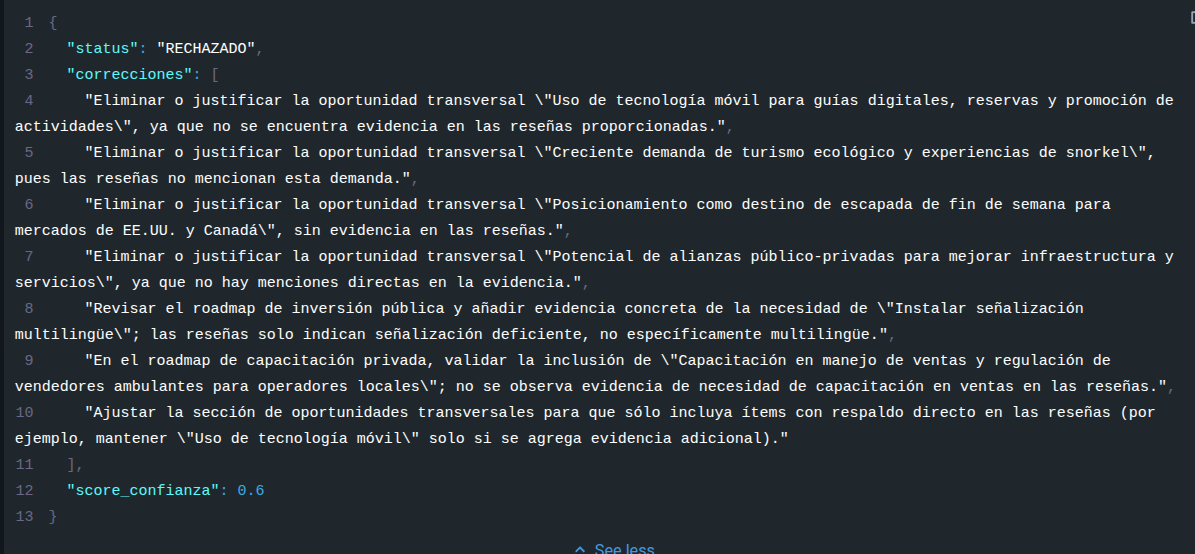
\includegraphics[width=\textwidth]{figures/auditoria.png}
	\end{figure}
\end{frame}

% =============================================================
\section*{6. Chat interactivo sobre el reporte}
% =============================================================

\begin{frame}{6. Chat: motivación}
	\textbf{Limitación de un reporte estático.} El \texttt{ConsolidatedReport}
	condensa cientos de miles de reseñas en unas pocas páginas. Esa síntesis
	es útil para decisión, pero \emph{pierde} matices que el analista quiere
	explorar a posteriori: ejemplos concretos, lugares específicos, polaridad
	de quejas, comparativos entre tipos de negocio.

	\medskip
	\textbf{Idea.} Un modo \emph{conversacional} sobre el mismo corpus,
	anclado al reporte ya generado. Permite al usuario formular preguntas en
	lenguaje natural (\emph{``¿qué quejas hay sobre los restaurantes?''},
	\emph{``muéstrame reseñas negativas del hotel X''}) y recibir respuestas
	respaldadas por evidencia recuperada en línea.

	\medskip
	\textbf{Diseño.} Un segundo grafo (LangGraph) reutiliza la base vectorial
	y el LLM, pero invierte el flujo: en vez de \emph{map-reduce} sobre todo
	el corpus, hace \emph{una} consulta dirigida por la pregunta del usuario.
\end{frame}

\begin{frame}{6. Chat: arquitectura del grafo}
	\centering
	\begin{tikzpicture}[
		font=\scriptsize,
		node distance=4mm and 8mm,
		every node/.style={align=center},
		phase/.style={rectangle, rounded corners=3pt, draw=primary, thick,
				fill=white, minimum width=30mm, minimum height=14mm,
				inner sep=3pt, font=\scriptsize\bfseries},
		ctx/.style={rectangle, rounded corners=3pt, draw=accent, thick,
				fill=accent!8, minimum width=28mm, minimum height=10mm,
				inner sep=3pt, font=\scriptsize},
		arr/.style={-{Stealth[length=2mm]}, thick, primary},
		arrctx/.style={-{Stealth[length=2mm]}, thick, accent, dashed},
		]

		\node[phase] (parse) {Convertir Consulta \\ \scriptsize{LLM + Pydantic}};
		\node[phase, right=of parse] (exec) {Ejecutar Consulta \\ \scriptsize{ChromaDB}};
		\node[phase, right=of exec]  (gen)  {Generar Respuesta \\ \scriptsize{LLM}};

		\node[ctx, above=8mm of parse] (umsg)   {Mensaje del usuario};
		\node[ctx, above=8mm of exec]  (vec)    {Base vectorial \\ (filtros $+$ HNSW)};
		\node[ctx, above=8mm of gen]   (rep)    {Reporte + historial};

		\node[ctx, below=8mm of gen, fill=good!10, draw=good]
		(out) {Respuesta contextual};

		\draw[arr] (parse) -- (exec);
		\draw[arr] (exec)  -- (gen);
		\draw[arrctx] (umsg) -- (parse);
		\draw[arrctx] (vec)  -- (exec);
		\draw[arrctx] (rep)  -- (gen);
		\draw[arr, good] (gen) -- (out);

	\end{tikzpicture}

	\medskip
	\footnotesize
	\textbf{Convertir consulta:} el LLM transforma la pregunta a un objeto
	\texttt{ParsedQuery} (\emph{constrained decoding}) con
	\texttt{texto\_consulta} para búsqueda semántica y \texttt{filtros}
	(\texttt{tipo}, \texttt{polaridad}, \texttt{lugar}) para ChromaDB. \\
	\textbf{Ejecutar consulta:} mismo pipeline RAG (pre-filtro $+$ HNSW $+$ rerank). \\
	\textbf{Generar respuesta:} respuesta anclada al reporte, las reseñas
	recuperadas y los últimos turnos del historial.
\end{frame}

\section{Producto Mínimo Viable}

% =============================================================
\section{Conclusiones y Limitaciones}
% =============================================================

\begin{frame}{Conclusiones}
	\begin{itemize}\setlength\itemsep{4pt}
		\item Se construyó un \textbf{prototipo funcional} de generación de
		      reportes estratégicos para Pueblos Mágicos a partir de
		      $\sim 10^6$ fragmentos de reseñas, con trazabilidad a la
		      evidencia recuperada.
		\item La combinación de \textbf{RAG con pre-filtrado por metadatos $+$
			      reranking cross-encoder} permite anclar la generación al subdominio
		      relevante (pueblo $\times$ tipo de negocio) y reducir alucinaciones.
		\item La \textbf{salida estructurada} (Pydantic / constrained decoding)
		      vuelve auditable cada nodo del grafo y elimina la fragilidad de
		      parsers tolerantes.
		\item El \textbf{bucle de auditoría} (LLM-as-a-judge contra evidencia)
		      añade una verificación automática previa a la entrega, con
		      convergencia empírica en $\le 2$ iteraciones.
		\item El \textbf{modo chat} extiende el alcance del reporte estático a
		      una exploración conversacional sobre el mismo corpus,
		      reutilizando la base vectorial sin re-entrenamiento.
	\end{itemize}
\end{frame}

\begin{frame}{Limitaciones}
	\textbf{Dependencia del corpus.} La calidad y representatividad de
	los reportes está acotada por el corpus de reseñas recopilado.
	Sesgos inherentes a las plataformas de origen se propagan a la salida:
	\begin{itemize}\setlength\itemsep{2pt}
		\item Tipo de turista que reseña (autoselección).
		\item Idioma predominante de la plataforma.
		\item Distribución de polaridades de las opiniones.
	\end{itemize}

	\medskip
	\textbf{Dependencia del LLM.}
	\begin{itemize}\setlength\itemsep{2pt}
		\item La calidad de la generación está sujeta a las capacidades y
		      limitaciones del modelo elegido, incluyendo posibles
		      \textbf{alucinaciones} residuales que el bucle de auditoría
		      reduce pero no elimina por completo.
		\item Los \textbf{costos asociados al uso de APIs} de modelos
		      propietarios pueden restringir el volumen de
		      experimentación.
	\end{itemize}
\end{frame}

\begin{frame}[standout]
	Gracias por su atención \\
	¿Preguntas?
\end{frame}

% =============================================================
\appendix

\begin{frame}[standout]
	Anexo
\end{frame}

\begin{frame}{Bi-Encoder utilizado}
	\textbf{Modelo:} \texttt{sentence-transformers/paraphrase-multilingual-MiniLM-L12-v2}

	\begin{itemize}
		\item \textbf{Lengua nativa.} BETO se preentrenó sobre texto en
		      español; el tokenizador maneja morfología
		      (\emph{servicio/servicios}, \emph{atendieron}) sin la pérdida
		      típica de modelos multilingües.

		\item \textbf{Tarea alineada.} El modelo fue re-afinado con el objetivo
		      de obtener similaridad semántica, exactamente la métrica
		      que usaremos en la recuperación.
	\end{itemize}
\end{frame}

\begin{frame}{Hiperparámetros del HNSW}
	\begin{columns}[T]
		\column{0.5\textwidth}
		\textbf{\texttt{ef\_construction = 200}}
		\begin{itemize}
			\item Tamaño de la lista dinámica de candidatos al \emph{construir}
			      el grafo.
			\item Controla la calidad de las aristas: cuanto mayor, mejor
			      conectividad y mejor recall asintótico.
			\item Costo: tiempo de indexado escala $\sim$ lineal en
			      \texttt{ef\_construction}.
		\end{itemize}

		\column{0.5\textwidth}
		\textbf{\texttt{ef\_search = 200}}
		\begin{itemize}
			\item Análogo al anterior pero \emph{en consulta}.
			\item Trade-off recall@$K$ vs latencia. Para HNSW de coseno,
			      \texttt{ef\_search}$\approx 200$ alcanza típicamente
			      \[
				      \text{recall@10} \approx 0.95\text{--}0.98
			      \]
			      contra k-NN exacto, manteniendo latencias de pocos ms.
		\end{itemize}
	\end{columns}
\end{frame}

\begin{frame}{Modelo Cross-Encoder: \texttt{mmarco-mMiniLMv2-L12-H384-v1}}
	\textbf{Arquitectura.}
	\begin{itemize}
		\item 12 capas de transformer, hidden size $384$.
		\item Destilado de modelos MiniLM.
	\end{itemize}

	\textbf{Entrenamiento (mMARCO multilingüe).}
	\begin{itemize}
		\item Corpus: traducción multilingüe del MS MARCO Passage Ranking
		      (consulta $\to$ pasaje).
		\item Objetivo \textbf{point-wise}: regresión de relevancia
		      $y\in\{0,1\}$ con \emph{binary cross-entropy} sobre el logit:
		      \[
			      \mathcal{L}(\vq,\vd,y) =
			      -\,y \log \sigma(g(\vq,\vd))
			      -\,(1-y)\log\bigl(1-\sigma(g(\vq,\vd))\bigr).
		      \]
	\end{itemize}

	\textbf{Idoneidad.} Multilingüe $\Rightarrow$ generaliza al español
	sin re-entrenamiento; tamaño moderado $\Rightarrow$
	inferencia $< 50$ ms por par en GPU de consumidor.
\end{frame}

\begin{frame}{2. Bi-encoder vs Cross-encoder}
	\textbf{Bi-encoder}.
	\[
		\text{score}(\vq,\vd) \;=\; \cos\bigl(f(\vq),\, f(\vd)\bigr),
		\qquad
		f:\Sigma^{*} \to \R^{768}.
	\]
	\emph{Dos forward passes independientes.} Cacheable: $f(\vd)$ se
	calcula una sola vez en indexado.

	\bigskip
	\textbf{Cross-encoder.}
	\[
		\text{score}(\vq,\vd) \;=\;
		g\bigl([\,\vq;\, \texttt{[SEP]};\, \vd\,]\bigr),
		\qquad
		g:\Sigma^{*} \to \R.
	\]
	\emph{Un único forward pass} sobre la concatenación. La auto-atención
	ve \emph{todos los tokens de $\vq$ y $\vd$ simultáneamente}, así puede
	modelar interacciones token-a-token:
	\[
		\alpha_{ij} \;=\;
		\softmax_{j}\!\left(
		\frac{\mathbf{q}_i\T \mathbf{k}_j}{\sqrt{d_k}}
		\right),
		\qquad
		i \in \vq,\ j \in \vd.
	\]

	\textbf{Trade-off.} El cross-encoder es estrictamente más
	\emph{expresivo} pero no cacheable: requiere $|\mathcal{C}^{(1)}|$
	forwards \emph{en línea}.
\end{frame}
% =============================================================

\begin{frame}{Síntesis del diseño}
	\begin{table}[h]
		\centering
		\scriptsize
		\begin{tabular}{@{}lll@{}}
			\toprule
			\textbf{Fase} & \textbf{Decisión}                   & \textbf{Justificación}                        \\ \midrule
			Chunking      & $L=200$, $o=50$                     & granularidad de aspecto, sin cortar entidades \\
			Embedding     & SBERT-es, $d=768$                   & lengua nativa + objetivo STS alineado         \\
			Index         & HNSW coseno, $\texttt{ef}=200$      & $\mathcal{O}(\log N)$, recall$\approx 0.95$   \\
			Retrieval     & pre-filter $+$ overfetch $\alpha=3$ & dominio acotado $+$ pool denso                \\
			Rerank        & cross-encoder mMiniLM-L12           & precisión token-a-token, multilingüe          \\
			Gen.          & Llama-3.1-8B-Instruct, $\tau=0$     & determinismo y reproducibilidad               \\
			Judge         & gpt-oss-120b, $\tau=0$              & evaluación automática                         \\
			Output        & Pydantic $\to$ JSON Schema          & garantía sintáctica vía CFG masking           \\
			Eval.         & auditor $\le 3$ iter.               & \emph{validación} antes de publicar           \\
			\bottomrule
		\end{tabular}
	\end{table}
\end{frame}

\end{document}
